\subsection{Descrição de \textit{software}}\label{subsec:software}

\begin{figure*}[!htpb]
\centering
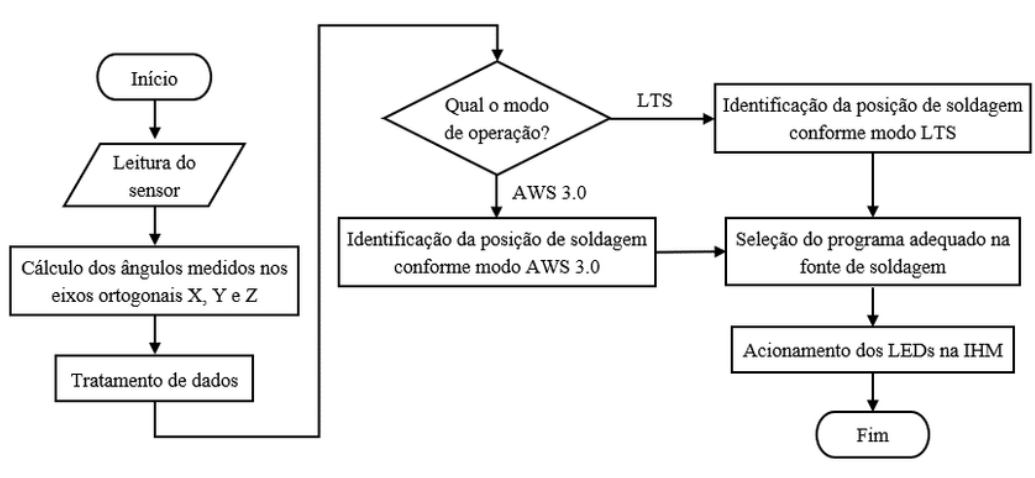
\includegraphics[width=.8\textwidth]{figuras/exemplo_de_fluxograma.png}
\caption{Exemplo de fluxograma~\cite{ref:exemplo_fluxograma}.}
\label{fig:exemplo_fluxograma}
\end{figure*}

Explique textualmente o algoritmo desenvolvido.
Esta subseção do relatório \textbf{NÃO CONSISTE} em simplesmente replicar o código, e sim em explicar como ele funciona, justificando suas escolhas de projeto.
O código pode ser apresentado como um apêndice ao relatório. 

Utilize fluxogramas como o da Fig. \ref{fig:exemplo_fluxograma} para auxiliar no entendimento do algoritmo desenvolvido.
Repare que a figura ocupa as duas colunas, usando o comando \verb|\begin{figure*} \end{figure*}| ao invés de \verb|\begin{figure} \end{figure}|.

Tópicos importantes a serem descritos nesta Subseção incluem:

\begin{itemize}
    \item \textbf{Coleta de dados:} conexão com sensores, definição da taxa de amostragem etc.
    \item \textbf{Processamento de dados:} filtro média-móvel, detecção de faces, reconhecimento de caracteres etc.	
    \item \textbf{Atuadores:} PWM, escrita em \textit{drivers} etc.	
    \item \textbf{Armazenamento/transmissão:} salvar em arquivo, enviar para a nuvem etc.	
    \item \textbf{Interface com o usuário:} GUI, interrupções para botões etc.
    \item \textbf{Inserção do programa no sistema operacional:} inicialização automática (\textit{crontab}, \texttt{/etc/init.d}), desligamento de serviços desnecessários, \textit{Buildroot} etc.
\end{itemize}